\documentclass[11pt]{article}

\input{../../preamble.tex}

\usepackage[margin=1in]{geometry}
\usepackage{amsmath,amssymb,bm}
\usepackage{graphicx}
\usepackage{float}
\usepackage{setspace}
\usepackage{tikz}
\usepackage{ulem}
\usetikzlibrary{calc}

% ---------- Small helpers ----------
\newcommand{\kb}[1]{\bm{k}_{#1}}
\newcommand{\ob}[1]{\bm{o}_{#1}}
\newcommand{\vb}{\bm{v}}
\newcommand{\wb}{\bm{\omega}}
\newcommand{\J}{\bm{J}}
\newcommand{\q}{\bm{q}}
\newcommand{\qd}{\dot{\bm{q}}}
\newcommand{\twist}{\begin{bmatrix}\vb\\ \wb\end{bmatrix}}
\newcommand{\utilde}[1]{\underset{\sim}{#1}}

\begin{document}

\begin{center}

{\Large University of British Columbia}

\vspace{0.2cm}

MECH 464/563 EECE 442/589: Introduction to Robotics

\vspace{0.1cm}

{\large Assignment \#9}

\vspace{0.1cm}

Dominic Klukas SN 64348378

\end{center}

\vspace{1em}

\noindent\textbf{Exercise \# 1:}
\begin{enumerate}
    \item[(a)] Prove the Huygens-Steiner formula (p.\ 65, equation (26)), Dynamics notes, ch6\_dynamics-1.pdf.
    \item[(b)] Obtain a body-coordinates version of Euler's equation (p.\ 68, equation (52)) from your dynamics notes with the inertia matrix being replaced with its representation in body-attached frame, a constant.
\end{enumerate}


\vspace{1em}

\begin{enumerate}
    \item[(a)] We fix a co-ordinate system $\{\utilde{o}_0, \underline{C}_0\}$.
        Let $\{\utilde{o}, \underline{C}\}$ be any other co-ordinate system.
        Then, as was derived in the notes (equation (16) page 64)
        \begin{align*}
            \underline{\mu}_{\utilde{o}_{0}} &=  m(\utilde{c} - \utilde{o}) \times  \dot{\utilde{o}} + (\utilde{o} - \utilde{o}_0) \times \underline{p} + \uuline{J}_{\utilde{o}} \uline{\omega}
        .\end{align*}

        However, applying this equation to the co-ordinate system $\{\utilde{o}, \uline{C}\} $, we get:
        \begin{align*}
            \underline{\mu}_{\utilde{o}_{0}} &=   (\utilde{c} - \utilde{o}_0) \times \underline{p} + \uuline{J}_{\utilde{c}} \uline{\omega}
        .\end{align*}
        Now, $\dot{\utilde{o}} = \dot{\utilde{c}} + \uline{\omega} \times (\utilde{o} - \utilde{c})$, and $p = m \dot{\utilde{c}}$.
        Combining these equations, we get
        \begin{align*}
            m(\utilde{c} - \utilde{o}) \times  \dot{\utilde{o}} + (\utilde{o} - \utilde{o}_0) \times \underline{p} + \uuline{J}_{\utilde{o}} \uline{\omega}
            &= (\utilde{c} - \utilde{o}_0) \times \underline{p} + \uuline{J}_{\utilde{c}} \uline{\omega}\\
            \uuline{J}_{\utilde{o}} \uline{\omega} &= (\utilde{c} - \utilde{o}) \times \uline{p} - m(c - o) \times \dot{\utilde{o}} + \uuline{J}_{\utilde{c}}\underline{\omega}\\
            \uuline{J}_{\utilde{o}} \uline{\omega} &= (\utilde{c} - \utilde{o}) \times (m \dot{\utilde{c}}) - m(c - o) \times \dot{\utilde{o}} + \uuline{J}_{\utilde{c}}\underline{\omega}\\
            \uuline{J}_{\utilde{o}} \uline{\omega} &= m(\utilde{c} - \utilde{o}) \times (\dot{\utilde{o}} - \uline{\omega} \times  (\utilde{o} - \utilde{c})) - m(c - o) \times \dot{\utilde{o}} + \uuline{J}_{\utilde{c}}\underline{\omega}\\
            \uuline{J}_{\utilde{o}} \uline{\omega} &= m(\utilde{c} - \utilde{o}) \times (\dot{\utilde{o}} - \uline{\omega} \times  (\utilde{o} - \utilde{c}) - \dot{\utilde{o}}) + \uuline{J}_{\utilde{c}}\underline{\omega}\\
            \uuline{J}_{\utilde{o}} \uline{\omega} &= m(\utilde{c} - \utilde{o}) \times ( - \uline{\omega} \times  (\utilde{o} - \utilde{c})) + \uuline{J}_{\utilde{c}}\underline{\omega}\\
            \uuline{J}_{\utilde{o}} \uline{\omega} &= m(\utilde{c} - \utilde{o}) \times ( -  (\utilde{c} - \utilde{o}) \times  \uline{\omega}) + \uuline{J}_{\utilde{c}}\underline{\omega}\\
            \uuline{J}_{\utilde{o}} \uline{\omega} &=  - m(\utilde{c} - \utilde{o}) \times (\utilde{c} - \utilde{o}) \times  \uline{\omega} + \uuline{J}_{\utilde{c}}\underline{\omega}\\
            \uuline{J}_{\utilde{o}} \uline{\omega} &=  - m[(\utilde{c} - \utilde{o}) \times]^2 \uline{\omega} + \uuline{J}_{\utilde{c}}\underline{\omega}
        .\end{align*}
        Since $\underline{\omega}$ was arbitrary, so it holds for all $\uline{\omega}$, including a basis.
        Since these two sides match on a basis, they are the same linear operator by linearity, so we have
        \begin{equation*}
            \uuline{J}_{\utilde{o}} =\uuline{J}_{\utilde{c}}- m[(\utilde{c} - \utilde{o}) \times]^2 
        ,\end{equation*}
        as desired.
    \item[(b)] Starting with the Euler equation:
        \[
            \uuline{J}_{\utilde{c}} \dot{\uline{\omega}} + \uline{\omega} \times  \uuline{J}_{\utilde{c}} \uline{\omega} = \uline{\tau}_{\utilde{c}}
        ,\] 
        and also
        \[
            \uline{\tau}_{\utilde{o}} = \uline{\tau}_{\utilde{c}} + (\utilde{c} - \utilde{o}) \times  \dot{p}
        ,\] 
        we substitute the result from part (a) to get
        \begin{align*}
            (\uuline{J}_{\utilde{o}} + m[(\utilde{c} - \utilde{o}) \times ]^2) \dot{\uline{\omega}} + \uline{\omega} \times  (\uuline{J}_{\utilde{o}} + m[(\utilde{c} - \utilde{o}) \times ]^2)\uline{\omega} &= \uline{\tau}_{\utilde{o}} - (\utilde{c} - \utilde{o}) \times  \dot{p}\\
            \uuline{J}_{\utilde{o}} \dot{\uline{\omega}}+ m[(\utilde{c} - \utilde{o}) \times ]^2 \dot{\uline{\omega}} + \uline{\omega} \times \uuline{J}_{\utilde{o}} \uline{\omega} + \uline{\omega} \times  m[(\utilde{c} - \utilde{o}) \times ]^2\uline{\omega} + (\utilde{c} - \utilde{o}) \times (m\ddot{\utilde{c}}) &= \uline{\tau}_{\utilde{o}}
        .\end{align*}

        Now, we compute:
        \begin{align*}
            \ddot{\utilde{c}} &= \ddot{\utilde{o}} - \dot{\omega} \times (\utilde{o} - \utilde{c}) - \omega \times (\dot{\utilde{o}} - \dot{\utilde{c}})\\
            \ddot{\utilde{c}} &= \ddot{\utilde{o}} - \dot{\omega} \times (\utilde{o} - \utilde{c}) - \omega \times (\omega \times  (\utilde{o} - \utilde{c}))
        .\end{align*}
        Then,
        \begin{align*}
            (\utilde{c} - \utilde{o}) \times \dot{p} = m(\utilde{c} - \utilde{o}) \times \ddot{\utilde{o}}  - m[(\utilde{c} - \utilde{o}) \times ]^2 \dot{\uline{\omega}} + m(\utilde{c} - \utilde{o}) \times ( \uline{\omega} \times  (\uline{\omega} \times (\utilde{o } - \utilde{c})))
        .\end{align*}
        Let's process these cross product terms.
        The triple product:
        \begin{align*}
            (\utilde{c} - \utilde{o}) \times  (\uline{\omega} \times ( \uline{\omega} \times  (\utilde{o} - \utilde{c})) ) &= (\utilde{c} - \utilde{o}) \times (\uline{\omega}(\uline{\omega}\cdot (\utilde{o} - \utilde{c})) - (\utilde{o} - \utilde{c}) \|\uline{\omega}\|^2)\\
                                                                                                                           &=(\uline{\omega} \cdot (\utilde{o} - \utilde{c})) (\utilde{c} - \utilde{o}) \times  \uline{\omega}\\
                                                                                                                           &=-(\uline{\omega} \cdot (\utilde{c} - \utilde{o})) (\utilde{c} - \utilde{o}) \times  \uline{\omega}
        .\end{align*}
        Similarly, we compute:
        \begin{align*}
            \uline{\omega} \times ((\utilde{c} - \utilde{o}) \times  ((\utilde{c} - \utilde{o}) \times \uline{\omega}))) &=  \uline{\omega} \times  ((\utilde{c} - \utilde{o})((\utilde{c} - \utilde{o}) \cdot  \uline{\omega}) - \uline{\omega} \|\utilde{c} - \utilde{o}\|^2) \\
                                                                                                                         &= \uline{\omega} \times (\utilde{c} - \utilde{o}) ((\utilde{c} - \utilde{o}) \cdot  \uline{\omega}) \\
                                                                                                                         &= - (\uline{\omega} \cdot  (\utilde{c} - \utilde{o})) (\utilde{c} - \utilde{o}) \times  \uline{\omega}
        .\end{align*}
        Therefore,
        \[
        \uline{\omega} \times ((\utilde{c} - \utilde{o}) \times  ((\utilde{c} - \utilde{o}) \times \uline{\omega})))=
            (\utilde{c} - \utilde{o}) \times  (\uline{\omega} \times ( \uline{\omega} \times  (\utilde{o} - \utilde{c})) )
        .\] 
        Putting this all together, we have

        \begin{align*}
            \uuline{J}_{\utilde{o}} \dot{\uline{\omega}}+ m[(\utilde{c} - \utilde{o}) \times ]^2 \dot{\uline{\omega}} + \uline{\omega} \times \uuline{J}_{\utilde{o}} \uline{\omega} + \uline{\omega} \times  m[(\utilde{c} - \utilde{o}) \times ]^2\uline{\omega} + (\utilde{c} - \utilde{o}) \times (m\ddot{\utilde{c}}) &= \uline{\tau}_{\utilde{o}}\\
            \uuline{J}_{\utilde{o}} \dot{\uline{\omega}}+\uline{\omega} \times \uuline{J}_{\utilde{o}} \uline{\omega} + m[(\utilde{c} - \utilde{o}) \times ]^2 \dot{\uline{\omega}} + \uline{\omega} \times  m[(\utilde{c} - \utilde{o}) \times ]^2\uline{\omega}  \quad &   \\
           + m (\utilde{c} - \utilde{o}) \times \ddot{\utilde{o}}  - m[(\utilde{c} - \utilde{o}) \times ]^2 \dot{\uline{\omega}} + m(\utilde{c} - \utilde{o}) \times ( \uline{\omega} \times  (\uline{\omega} \times (\utilde{o } - \utilde{c}))) &=\\
           \uuline{J}_{\utilde{o}} \dot{\uline{\omega}}+\uline{\omega} \times \uuline{J}_{\utilde{o}} \uline{\omega} + (m[(\utilde{c} - \utilde{o}) \times ]^2 \dot{\uline{\omega}}-m[(\utilde{c} - \utilde{o}) \times ]^2 \dot{\uline{\omega}}) + m (\utilde{c} - \utilde{o}) \times \ddot{\utilde{o}} \quad &\\
           + m\uline{\omega} \times  (\utilde{c} - \utilde{o}) \times (\utilde{c} - \utilde{o}) \times  \uline{\omega} - m(\utilde{c} - \utilde{o}) \times ( \uline{\omega} \times  (\uline{\omega} \times (\utilde{o } - \utilde{c}))) &=\\
           \uuline{J}_{\utilde{o}} \dot{\uline{\omega}}+\uline{\omega} \times \uuline{J}_{\utilde{o}} \uline{\omega} + m (\utilde{c} - \utilde{o}) \times \ddot{\utilde{o}} &= \uline{\tau}_{\utilde{o}}
        .\end{align*}
        In conclusion, we have that
\[
           \uuline{J}_{\utilde{o}} \dot{\uline{\omega}}+\uline{\omega} \times \uuline{J}_{\utilde{o}} \uline{\omega} + m (\utilde{c} - \utilde{o}) \times \ddot{\utilde{o}} = \uline{\tau}_{\utilde{o}}
,\] 
which is then our body-attached frame version of Euler's equation.

\end{enumerate}

\vspace{1em}

\noindent\textbf{Exercise \# 2:} Consider the pendulum -- example 6.3.1 of page 84 of your notes.
\begin{enumerate}
    \item[(i)] Obtain a computed torque controller that places the closed-loop poles at $s = -1$.
    \item[(ii)] Obtain the torque $\tau_d(t)$ necessary to drive the pendulum along the following trajectory:
\end{enumerate}

\begin{equation}
\theta_d(t)=
\begin{cases}
\frac{\pi}{2} t^2, & \text{if } 0 \le t \le 1,\\[0.5em]
\pi - \frac{\pi}{2}(t-2)^2, & \text{if } 1 < t \le 2,\\[0.5em]
\pi, & \text{if } 2 < t.
\end{cases}
\end{equation}

\noindent Draw a diagram of a feedforward position controller for this trajectory.

\vspace{1em}

\begin{enumerate}
    \item[(i)] The dynamics are given by:
        \[
            ml^2 \ddot{\theta} + mgl \sin\theta = \tau
        .\] 
        Now, if $\tau$ has the form $\tau(\theta)= mgl \sin\theta + u(\theta)$, then we have a simpler system:
        \begin{align*}
            ml^2 \ddot{\theta} = u(\theta)
        .\end{align*}
        Thus, the open loop transfer function of this system is then $G(s) = \frac{1}{ml^2 s^2} $.
        $\frac{K(s)G(s)}{1 + K(s)G(s)}$, where $K(s)$ is the controller.
        Let $k(e)$ be a simple feedback controller, where $e = \theta_d - \theta$, and so:
        \[
            k(e) = k_p e + k_d \dot{e}, \quad K(s) = k_p + s k_d
        .\] 
        Then, we get the following transfer function, for a feedback controller:
        \[
        \frac{G(s)K(s)}{1 + G(s)K(s)} = \frac{\frac{k_d s+k_p}{ml^2 s^2}}{1 + \frac{k_d s+k_p}{ml^2 s^2}} =  \frac{k_d s+k_p}{ml^2 (s^2+\frac{k_d s}{ml^2} +\frac{k_p}{ml^2})}
        .\] 
        We want our poles to be $s=-1$ (both of them), so we need the polynomial in the denominator to have the form $s^2 + 2s + 1$.
        This means that we need $k_d = 2 ml^2$, and $k_p = ml^2$.
        Therefore, our feedback controller is
        \[
            \tau(\theta, \dot{\theta}) = mgl \sin\theta - 2 ml^2 \dot{\theta} + ml^2(\theta_d - \theta)
        ,\] 
        where $\theta_d$ is the desired setpoint.
    \item[(ii)]
        Since we have that
        \[
            \tau = ml^2 \ddot{\theta} + mlg \sin\theta
        ,\] 
        we compute:
        \begin{align*}
            \dot{\theta_d} &= \begin{cases}
                \pi t, & \text{ if } 0 < t \leq 1,\\
                -\pi (t - 2),&\text{ if } 1 < t \leq 2,\\
                0, &\text{ if } 2 < t
            \end{cases}\\
            \ddot{\theta_d} &= \begin{cases}
                \pi & \text{ if } 0 < t \leq 1,\\
                -\pi, &\text{ if } 1 < t \leq 2,\\
                0, &\text{ if } 2 < t
            \end{cases}
        .\end{align*}
        Thus, we have that

        \[
        \tau_d(t) = \begin{cases}
            ml^2 \pi + mgl \sin(\frac{\pi}{2} t^2), & \text{ if } 0 \leq t < 1\\
            -ml^2 \pi + mgl \sin(\pi - \frac{\pi}{2}(t-2)^2), &\text{ if } 1 < t \leq 2\\
            0, &\text{ if } 2 < t
        \end{cases}
        .\] 

        For a feedforward position controller for this trajectory, we also include feedback terms, so that
        \[
            \tau(t) = \tau_d(t) + K_p (\theta_d(t) - \theta(t)) + K_v (\dot{\theta_d(t)} - \dot{\theta(t)})
        ,\] 
        which are tuned and adjusted.
        See figure \ref{fig:feedforward_controller}
        \begin{figure}[ht]
            \centering
            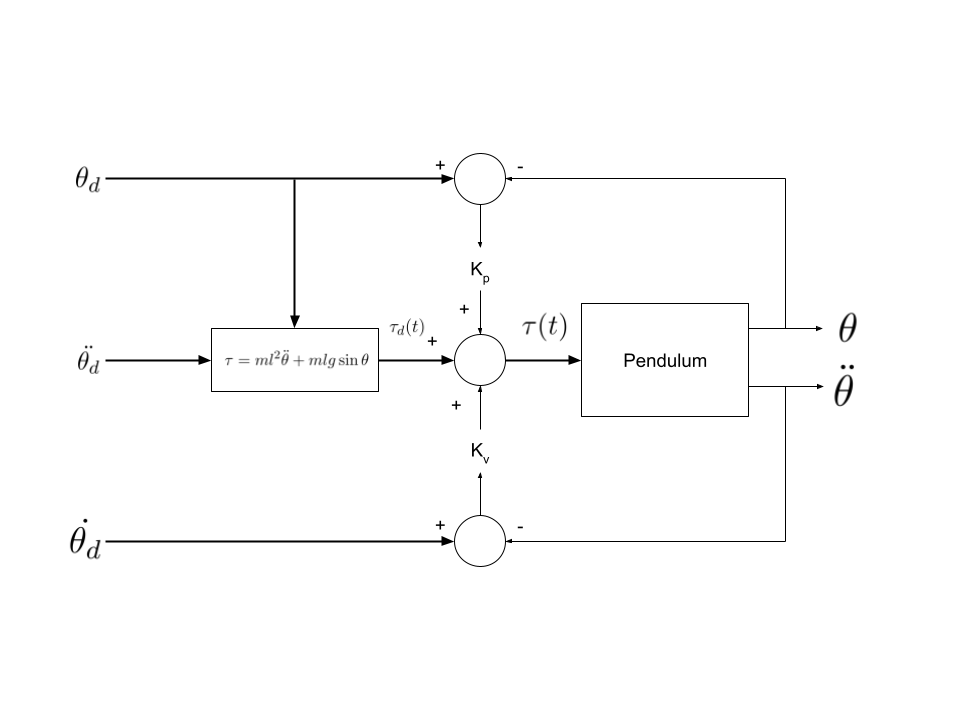
\includegraphics[width=0.7\linewidth]{2b.png}
            \caption{Feedforward position controller for trajecotry $\theta_d(t)$.}
            \label{fig:feedforward_controller}
    \end{figure}
\end{enumerate}

\vspace{1em}

\noindent\textbf{Exercise \# 3:}

\noindent Consider the two-link RR planar manipulator described in the dynamics section Ch.6, with
$l_1 = 1~\mathrm{m}$, $l_2 = 1~\mathrm{m}$, $m_1 = 1~\mathrm{kg}$, $m_2 = 1~\mathrm{kg}$.
The following Simulink model (uploaded on Canvas) simulates the PD+ gravity control of this manipulator.

\begin{figure}[H]
    \centering
    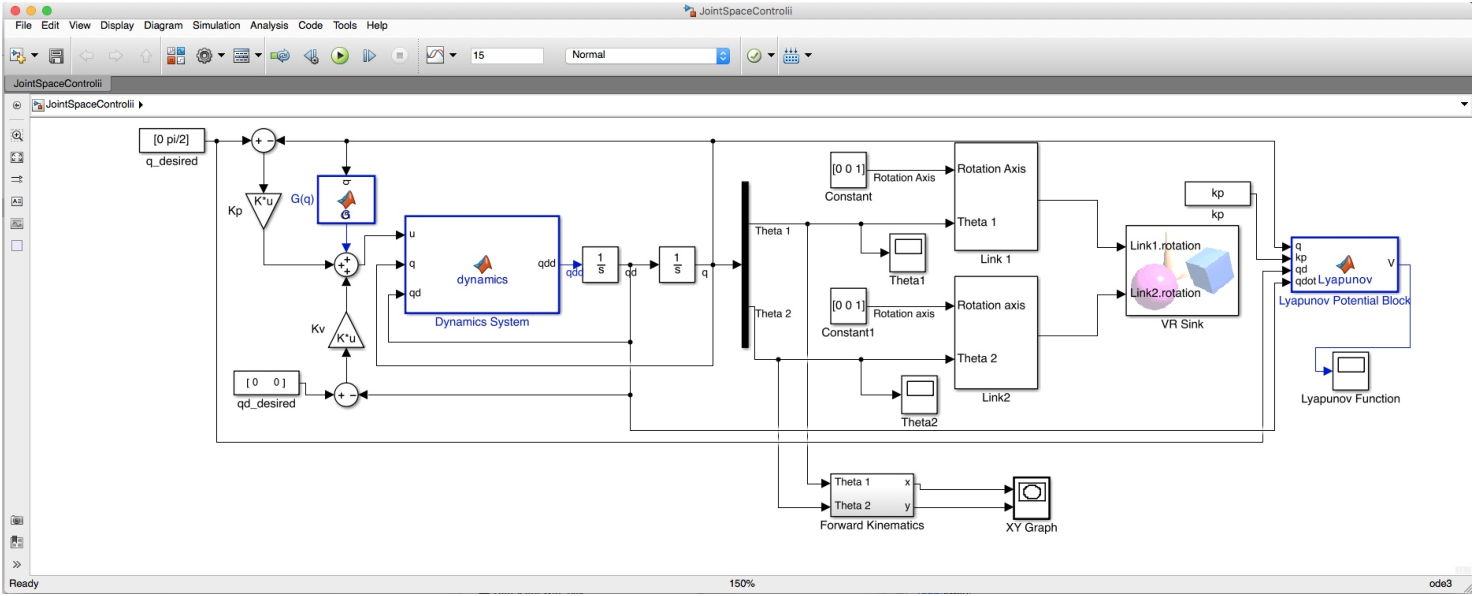
\includegraphics[width=\textwidth]{simulink.png}
\end{figure}

\noindent \textit{Open loop simulation.} Set the input torques to zero and simulate the open-loop system with different initial conditions.

\vspace{1em}

\noindent\textit{Closed loop cartesian space control.}

Design a ``stiffness'' controller and implement it using Simulink blocks. Demonstrate the response of the controller, for gains
$K_{p1} = \mathrm{diag}[1,1]$, $K_{p2} = \mathrm{diag}[0.2,1]$ and $K_{p3} = \mathrm{diag}[1,0.2]$,
with $K_v = \mathrm{diag}[2,2]$, simulating various spring directions in cartesian space.
Plot the end-effector trajectories from $t = 0$ to $t = 15~\mathrm{s}$, from the initial position
$q(0) = [\theta_1(0),\, \theta_2(0)]^T = [-\pi/2\ \ 0]^T$
(i.e.\ end effector at $\underset{\sim}{o}_0 - 0\,\underline{i}_0 - 2\,\underline{j}_0$
to $\underset{\sim}{o}_0 + 1\,\underline{i}_0 + 1\,\underline{j}_0$).


\textbf{Solution}

First, we investigate the open loop simulation. We delete the link between the sum output and the uinput of the dynamics system and input a constant instead.
Here are the results:

\begin{figure}[htbp]
    \centering

    % Row 1
    \begin{subfigure}[t]{0.45\textwidth}
        \centering
        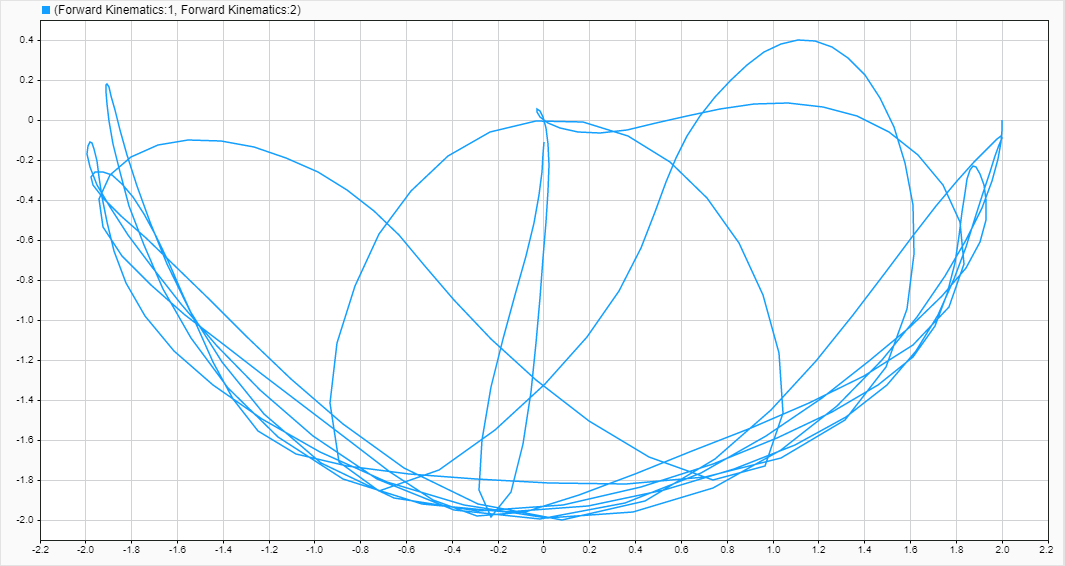
\includegraphics[width=\textwidth]{initial_position_pion20.png}
        \caption{Initial velocity: $0$, initial position: $(\pi/2, 0)$}
        \label{fig:init1}
    \end{subfigure}
    \hfill
    \begin{subfigure}[t]{0.45\textwidth}
        \centering
        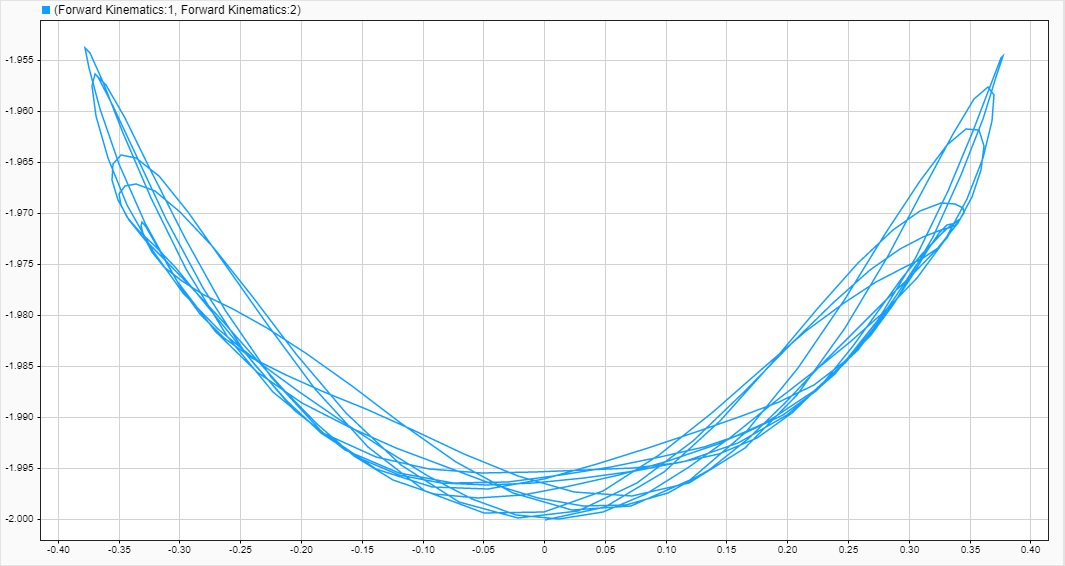
\includegraphics[width=\textwidth]{initial_velocity_01.png}
        \caption{Initial velocity: $(0,1)$, initial position: $(-\pi/2, 0)$}
        \label{fig:init2}
    \end{subfigure}

    \vspace{0.5em}

    % Row 2
    \begin{subfigure}[t]{0.45\textwidth}
        \centering
        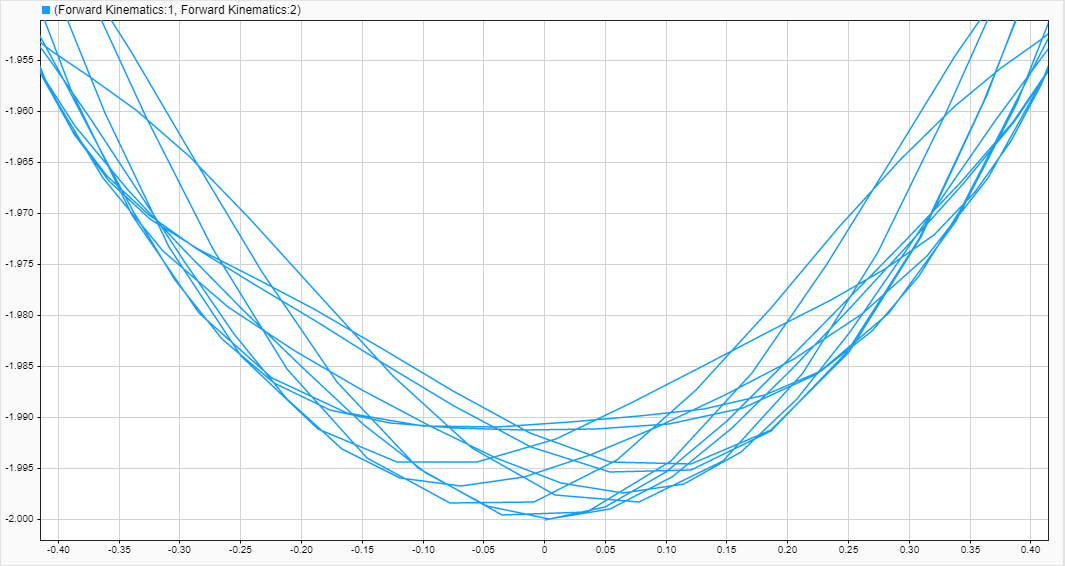
\includegraphics[width=\textwidth]{initial_velocity_1n1.png}
        \caption{Initial velocity: $(1,-1)$, initial position: $(-\pi/2, 0)$}
        \label{fig:init3}
    \end{subfigure}
    \hfill
    \begin{subfigure}[t]{0.45\textwidth}
        \centering
        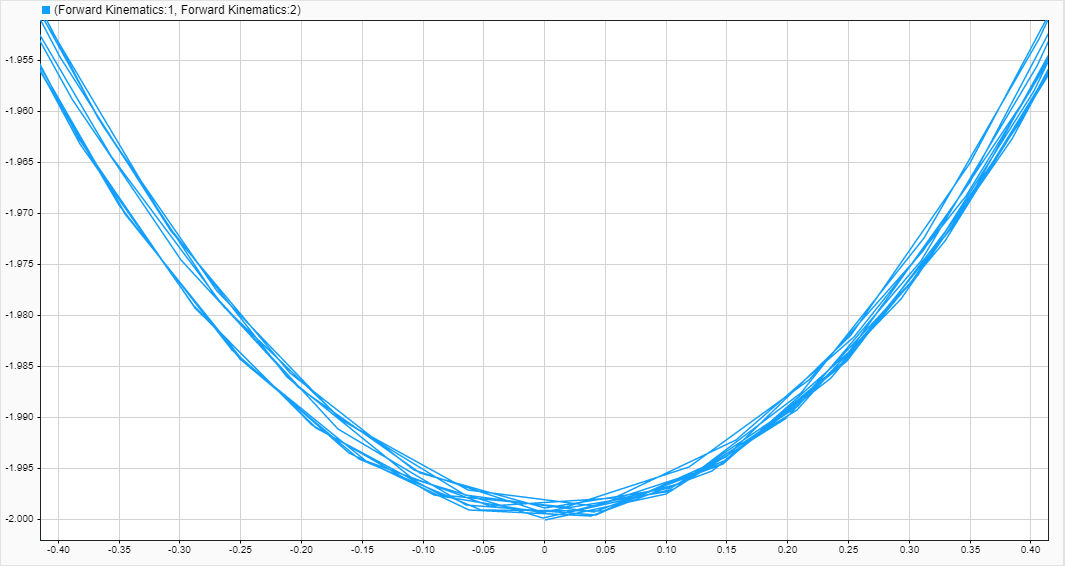
\includegraphics[width=\textwidth]{initial_velocity_10.png}
        \caption{Initial velocity: $(1,0)$, initial position: $(-\pi/2, 0)$}
        \label{fig:init4}
    \end{subfigure}

    \caption{System responses under different initial conditions.}
    \label{fig:initial_conditions}
\end{figure}

The open loop dynamic system with zero torque input obeys what we would expect from a physics simulation of a double pendulum.

For the stiffness controller, we build the controller using Simulink blocks as shown in \ref{fig:system}.
\begin{figure}[htbp]
    \centering
    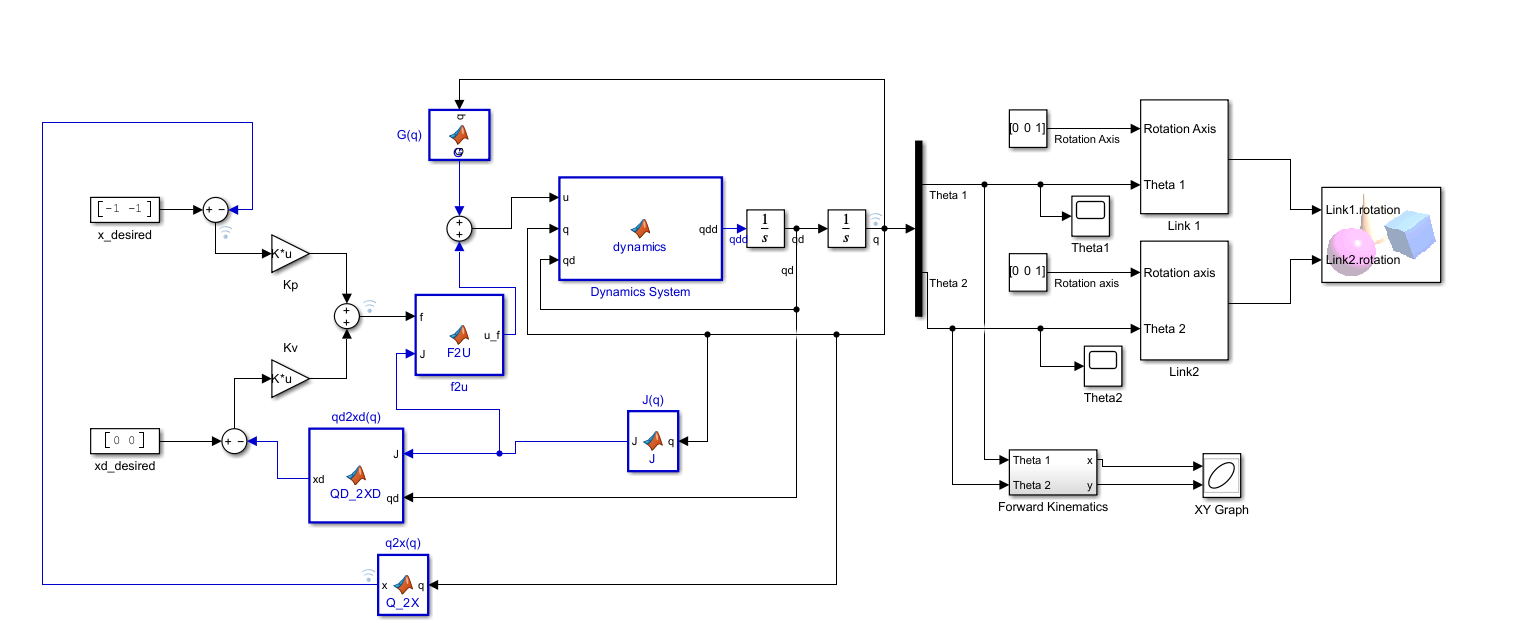
\includegraphics[width=0.8\textwidth]{system.png}
    \caption{PD + stiffness controller for a 2-joint pendulum system.}
    \label{fig:system}
\end{figure}

In particular, the following blocks implement the jacobian, convert the q to x values, and compute the joint torques from the cartesian force at the end effector, as shown in \ref{fig:blocks}.

\begin{figure}[htbp]
    \centering

    \begin{subfigure}[t]{0.32\textwidth}
        \centering
        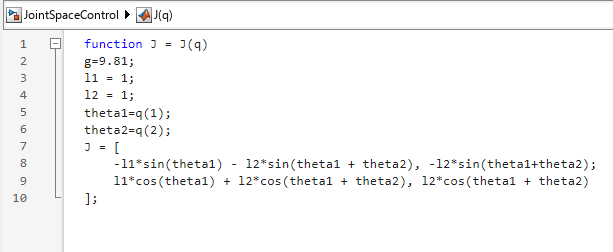
\includegraphics[width=\textwidth]{Jacobian.png}
        \caption{Jacobian computation}
        \label{fig:jacobian}
    \end{subfigure}
    \hfill
    \begin{subfigure}[t]{0.32\textwidth}
        \centering
        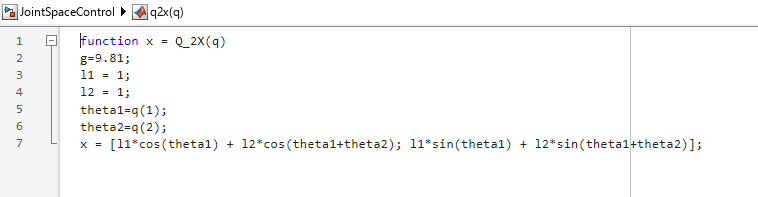
\includegraphics[width=\textwidth]{joint_to_coord.png}
        \caption{Joint to Cartesian mapping}
        \label{fig:joint_to_coord}
    \end{subfigure}
    \hfill
    \begin{subfigure}[t]{0.32\textwidth}
        \centering
        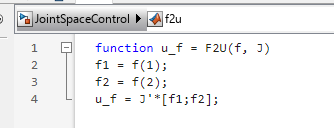
\includegraphics[width=\textwidth]{force_to_jointtorque.png}
        \caption{Force to joint torque}
        \label{fig:force_to_torque}
    \end{subfigure}

    \caption{Functional blocks used in the controller.}
    \label{fig:blocks}
\end{figure}

Finally, we demonstrate the response of the controller.
The first thing to note, is that we can run into issues with singularities.
For instance, when the pendulum is fully extened in it's stable bottomed out position, there is no way for the joints to make it go directly up.
So, if we set the desired position to be (0, 0) when the initial joint values are set to $(- \frac{\pi}{2}, 0)$, then we get the following trajectory, with the pendulum stuck in in it's bottom position (figure \ref{fig:stiffness_singularity}).

\begin{figure}[htbp]
    \centering
    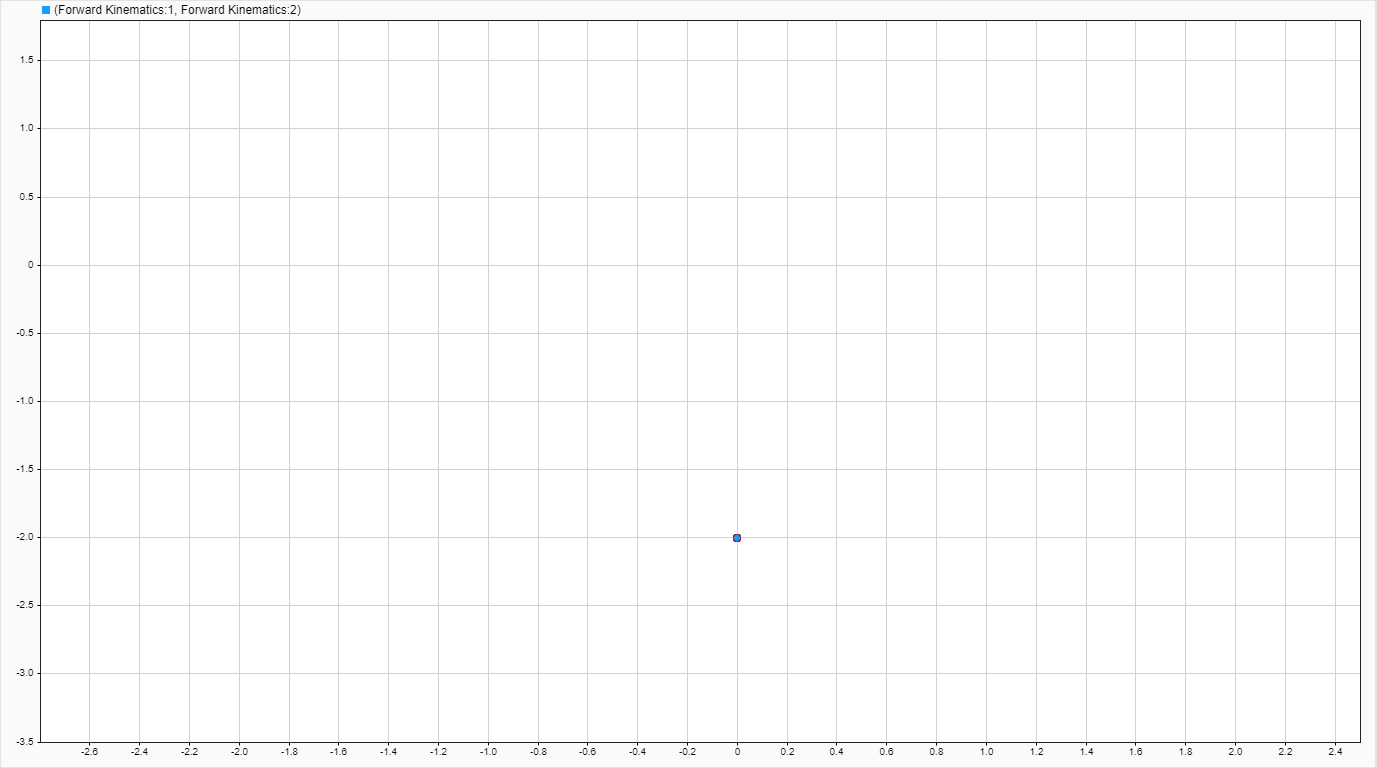
\includegraphics[width=0.7\textwidth]{stiffness_final00.png}
    \caption{Stiffness controller with desired position $(0,0)$ and initial position $(0,-2)$. The system becomes stuck due to a kinematic singularity, preventing the controller from generating a feasible motion toward the target.}
    \label{fig:stiffness_singularity}
\end{figure}

Next, we demonstrate the response of a trajectory from $\utilde{o}_{0} = 0 \uline{i}_0 - 2 \uline{j}$ to $\utilde{o} = 1 \uline{i}_0 + 1 \uline{j}_0$ for gains $K_{p1}, K_{p2}$ and $K_{p3}$ having $K_v$ fixed at $diag[2, 2]$.
See figure \ref{fig:stiffness_gains}.
Interesting is the case when we have high gain in the $y$ axis and low gain in the $x$ axis.
The high penatly in the $y$ direction gets the controller to greedily increase the $y$ momentum, and not penalize the resulting swing in the $x$ direction that happens as a result of the rotational nature of the system.
We also test a different ending point: $\utilde{o} = -1 \uline{i}_0 - 1 \uline{j}_0$.

\begin{figure}[htbp]
    \centering

    % -------- Row 1 --------
    \textbf{Target: $\utilde{o} = 1\uline{i}_0 + 1\uline{j}_0$}

    \begin{subfigure}[t]{0.32\textwidth}
        \centering
        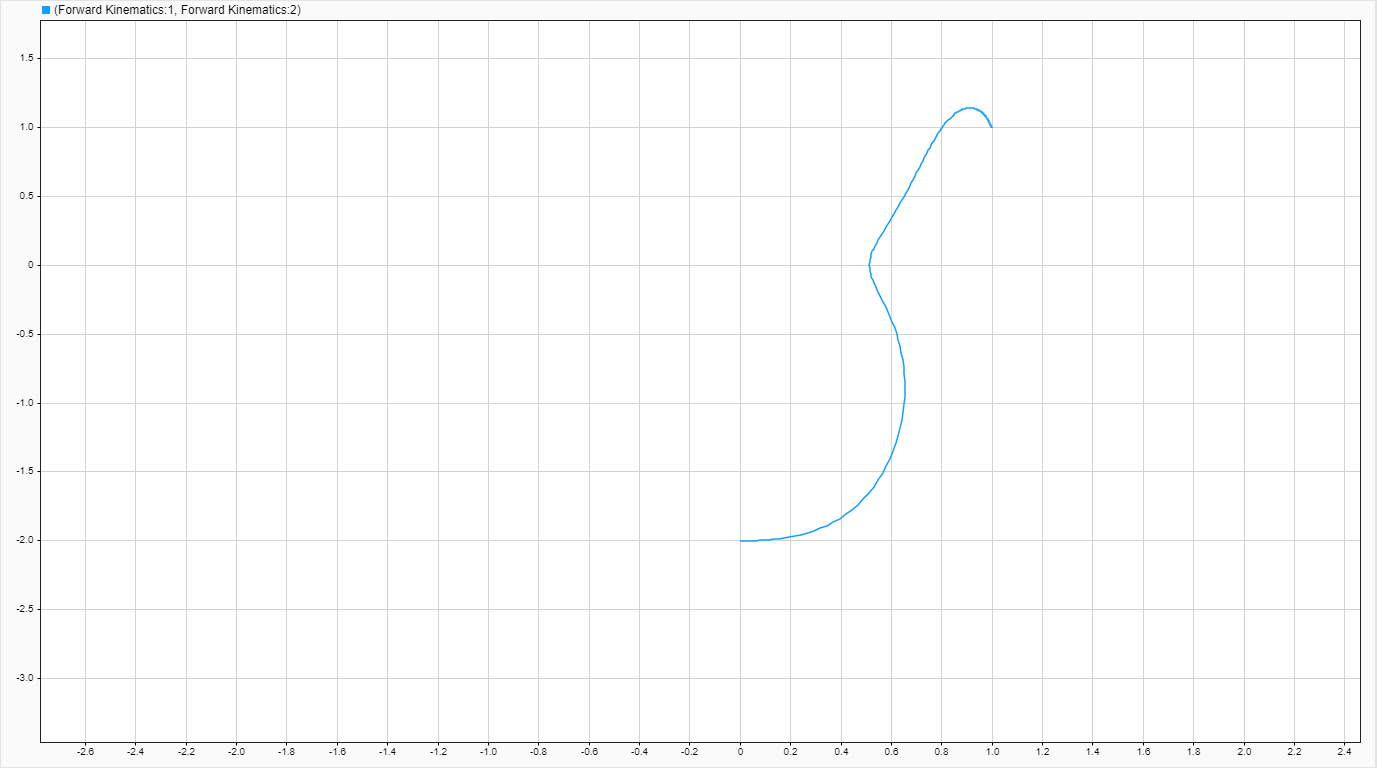
\includegraphics[width=\textwidth]{stiffness_K1.png}
        \caption{$K_{p1}=\mathrm{diag}[1,1]$}
    \end{subfigure}
    \hfill
    \begin{subfigure}[t]{0.32\textwidth}
        \centering
        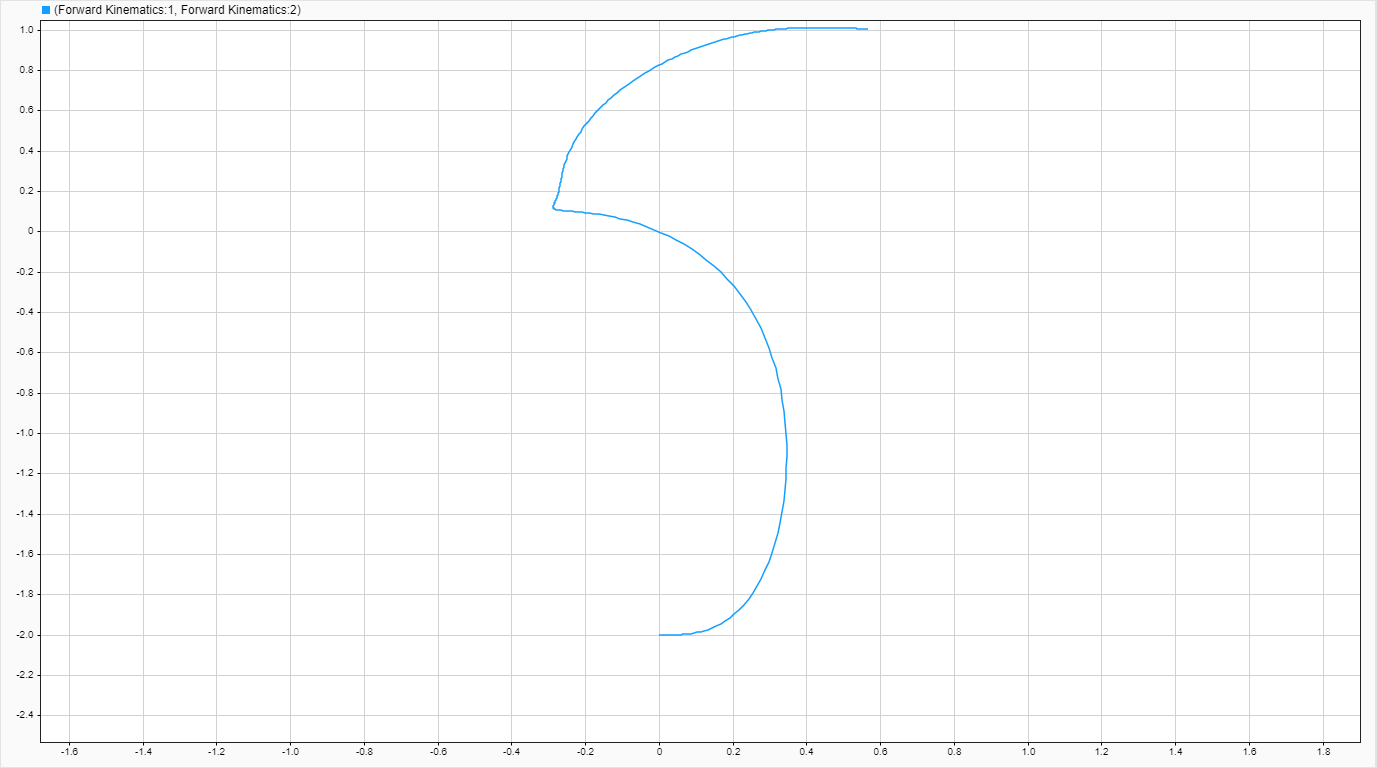
\includegraphics[width=\textwidth]{stiffness_K2.png}
        \caption{$K_{p2}=\mathrm{diag}[0.2,1]$}
    \end{subfigure}
    \hfill
    \begin{subfigure}[t]{0.32\textwidth}
        \centering
        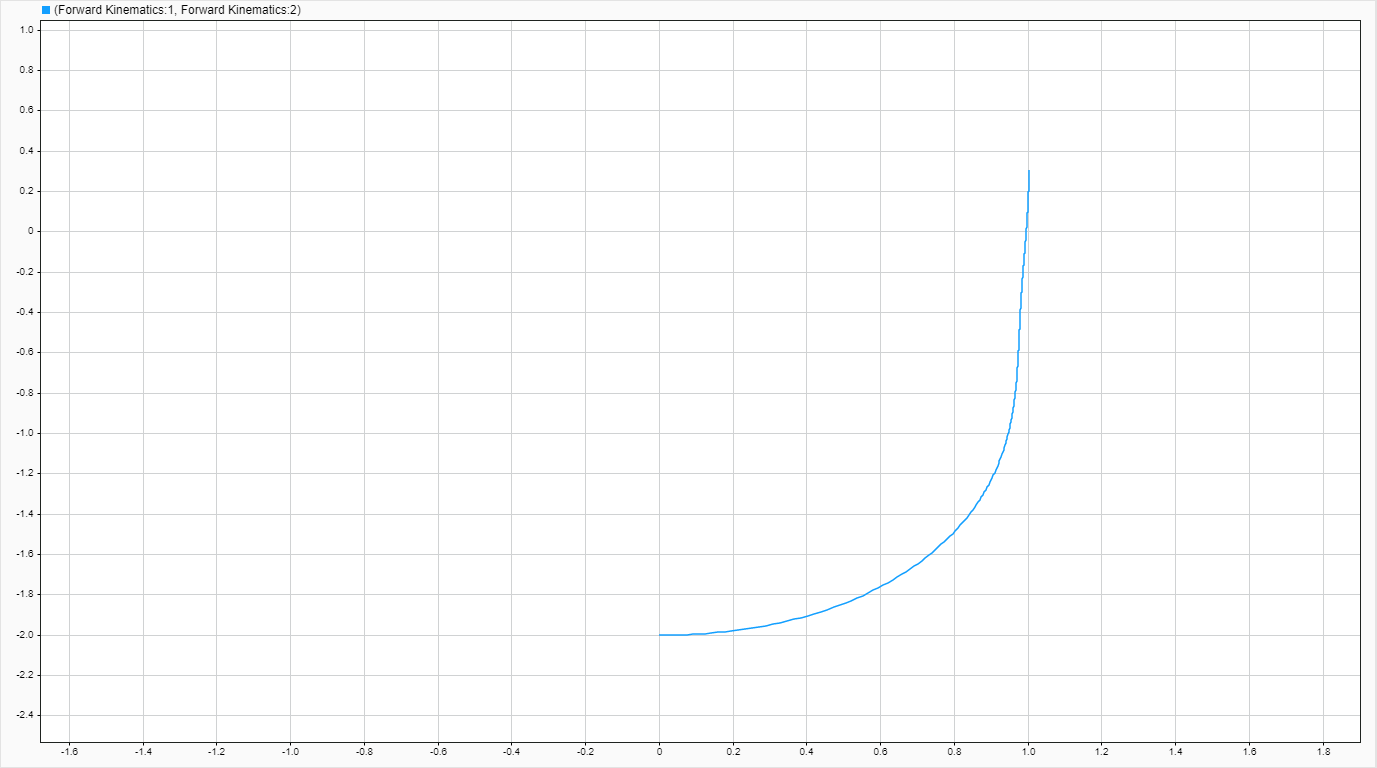
\includegraphics[width=\textwidth]{stiffness_Kp3.png}
        \caption{$K_{p3}=\mathrm{diag}[1,0.2]$}
    \end{subfigure}

    \vspace{1em}

    % -------- Row 2 --------
    \textbf{Target: $\utilde{o} = -1\uline{i}_0 - 1\uline{j}_0$}

    \begin{subfigure}[t]{0.32\textwidth}
        \centering
        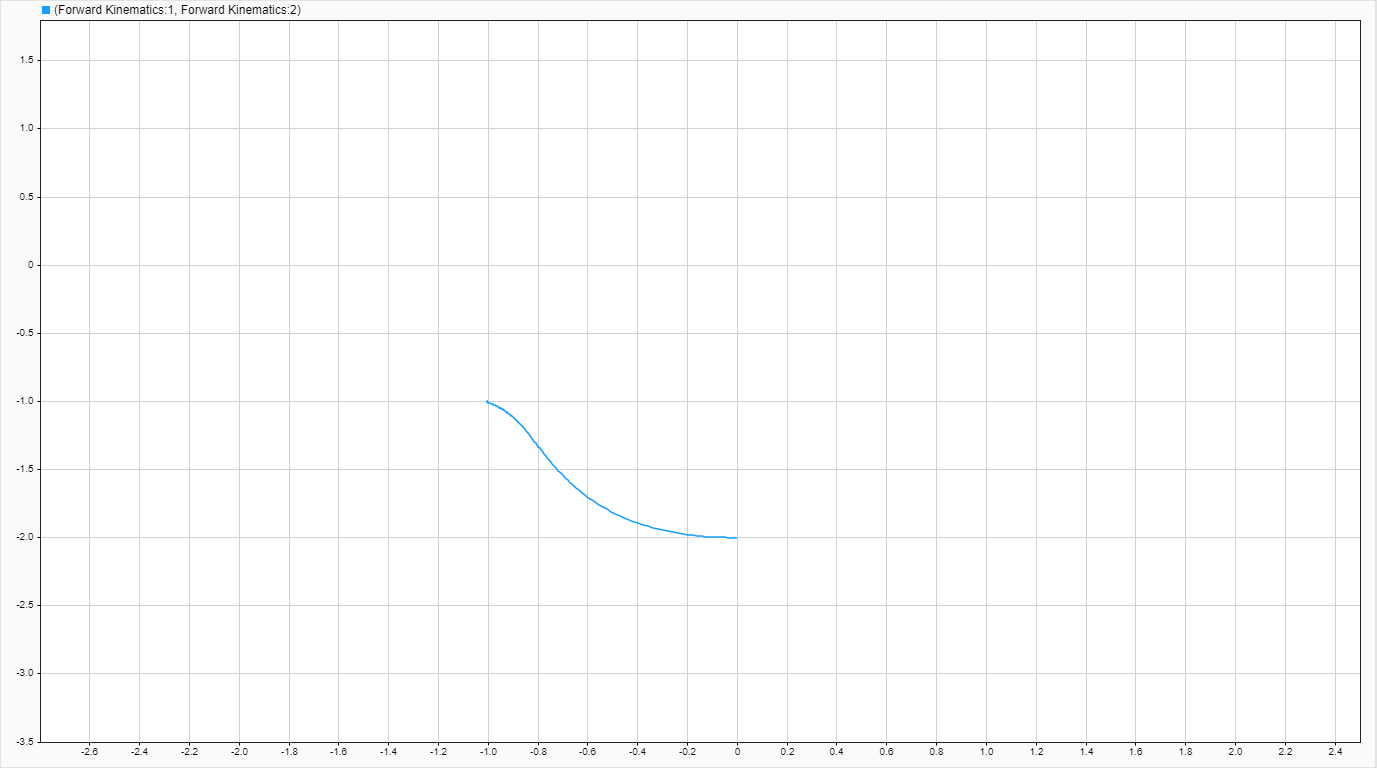
\includegraphics[width=\textwidth]{stiffness_n1n1_K1.png}
        \caption{$K_{p1}=\mathrm{diag}[1,1]$}
    \end{subfigure}
    \hfill
    \begin{subfigure}[t]{0.32\textwidth}
        \centering
        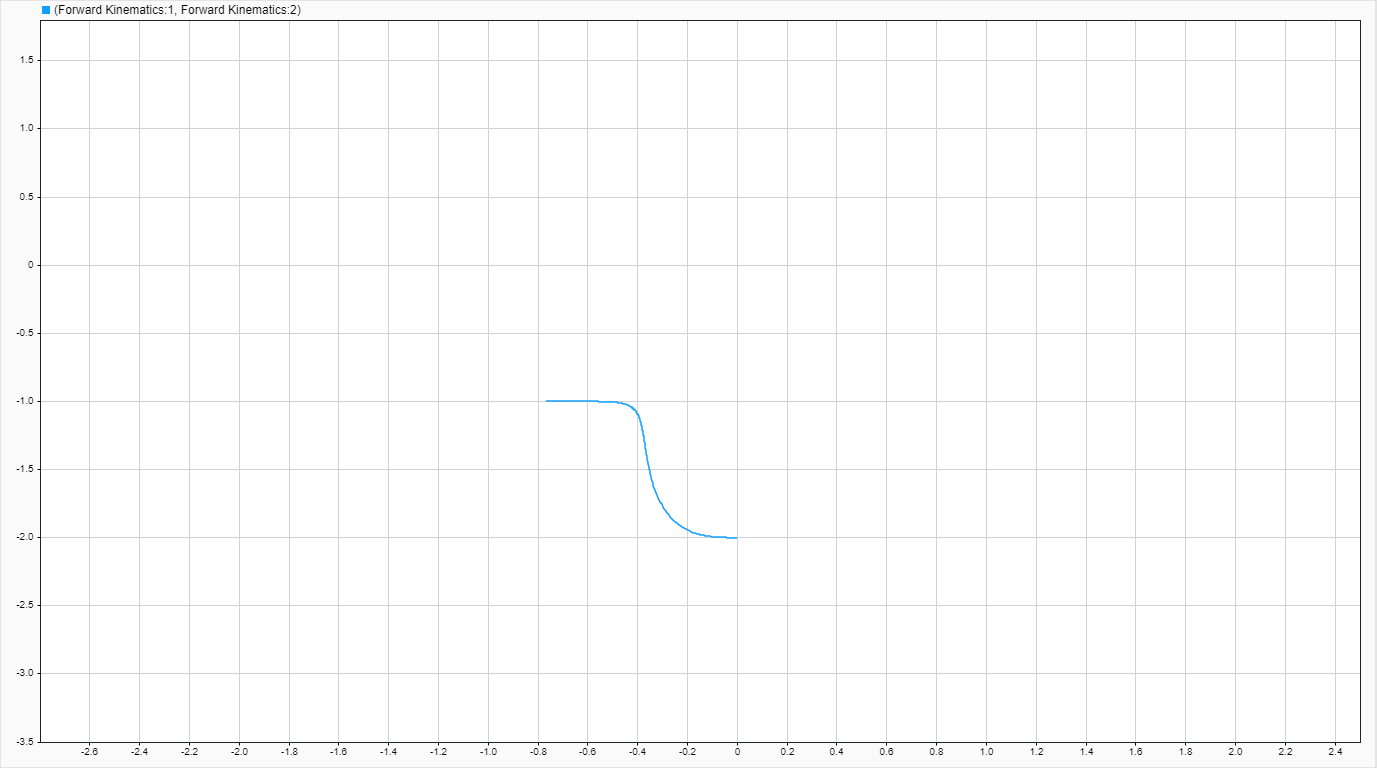
\includegraphics[width=\textwidth]{stiffness_n1n1_K2.png}
        \caption{$K_{p2}=\mathrm{diag}[0.2,1]$}
    \end{subfigure}
    \hfill
    \begin{subfigure}[t]{0.32\textwidth}
        \centering
        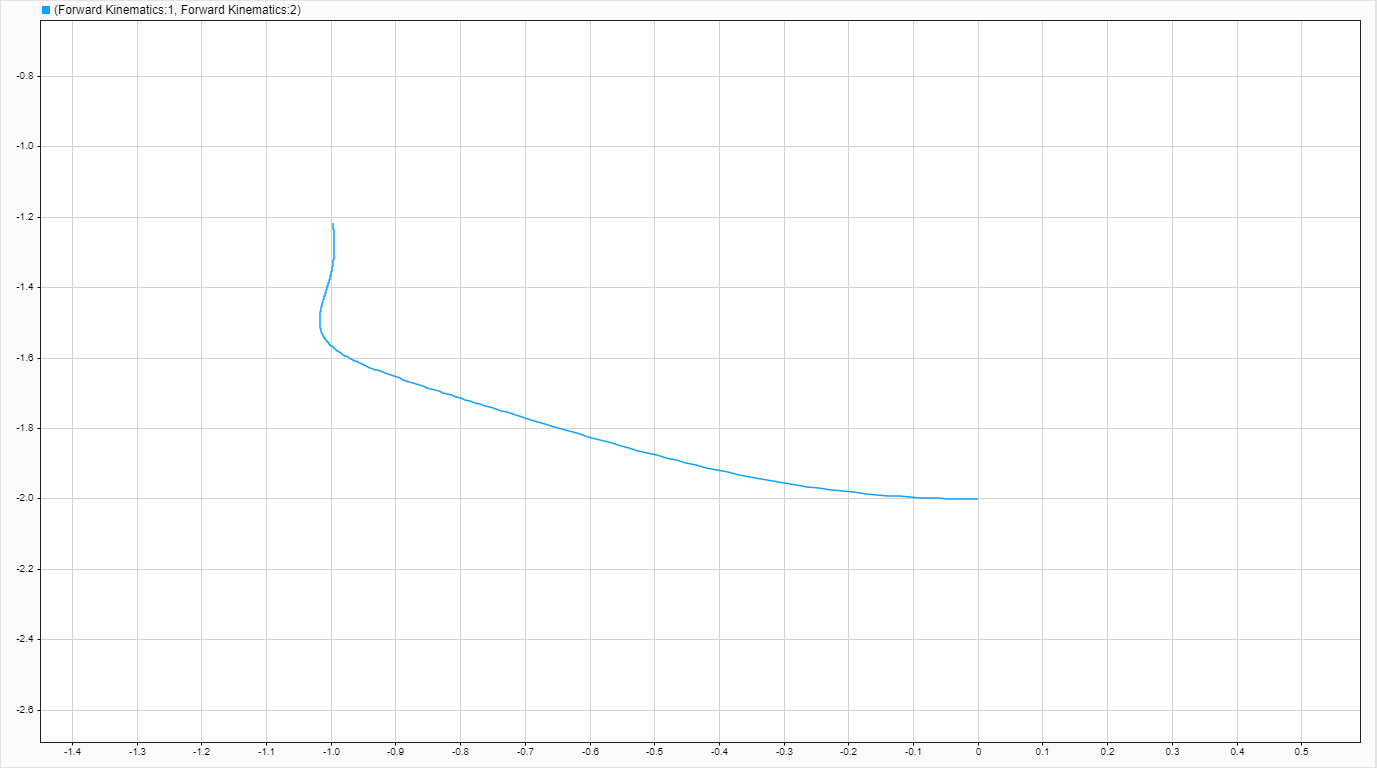
\includegraphics[width=\textwidth]{stiffness_n1n1_K3.png}
        \caption{$K_{p3}=\mathrm{diag}[1,0.2]$}
    \end{subfigure}

    \caption{End-effector trajectories under a stiffness controller from initial position $\utilde{o}_0 = 0\uline{i}_0 - 2\uline{j}_0$ with different stiffness gains. The top row shows motion toward $(1,1)$, while the bottom row shows motion toward $(-1,-1)$, illustrating how anisotropic gains influence the trajectory and effective spring direction in Cartesian space.}

    \label{fig:stiffness_gains}
\end{figure}

\end{document}
